\documentclass[UTF8]{ctexart}
\usepackage{multirow,amsmath,tikz,color}
\begin{document}
\begin{tabular}{ccc}
\hline
\multirow{2}{*}{Item} &\multicolumn{2}{c}{value} \\
\cline{2-3}
&first & second \\
a &b &c \\
\hline
\end{tabular}
$a^2+b^2=c^2$
\begin{equation}
a^2+b^2=c^2 \tag{123}\label{damd}
\end{equation}
cnsn \eqref{damd} cncnc \\
In text:
\[\lim_{n\to\infty} \sum_{k=1}^n \frac{1}{k^2}=\frac{\pi^2}{6}\] \\
$ \ne \ge \le \approx \equiv \propto \sim $  \\
\[a_1+a_2+\dots+a_n\]
$p_{ij}^3 \qquad m_{\text{mxm}}\quad \sum_{k=1}^3 k$\\
$f'(x)=x^2\quad f''^2(x)=2x$
\[\sqrt[4]{\pi^7} \quad \binom{n}{k}\quad \dim{3}\]\\
\[\lim_{x \rightarrow 0}\frac{\sin x}{x}=1\]
$ a,b,c \ne \{ a,b,c\} $
\[ \mathbf{X}= \left( \begin{array}{cccc}
x_{11} & x_{12} &\ldots &x_{1n} \\
x_{21} & x_{22} &\ldots &x_{2n} \\
\vdots & \vdots &\ddots &\vdots \\
x_{n1} & x_{n2} &\ldots &x_{nn}
\end{array} \right) \]
\[ |x|=\left\{  \begin{array}{lr}
-x & \text{if } x<0,\\
0 &\text{if } x=0,\\
x &\text{if } x>0.
\end{array}\right. \]
\[ \mathbf{X}=\begin{pmatrix}
x_{11} & x_{12} &\ldots &x_{1n} \\
x_{21} & x_{22} &\ldots &x_{2n} \\
\vdots & \vdots &\ddots &\vdots \\
x_{n1} & x_{n2} &\ldots &x_{nn}
\end{pmatrix} \]

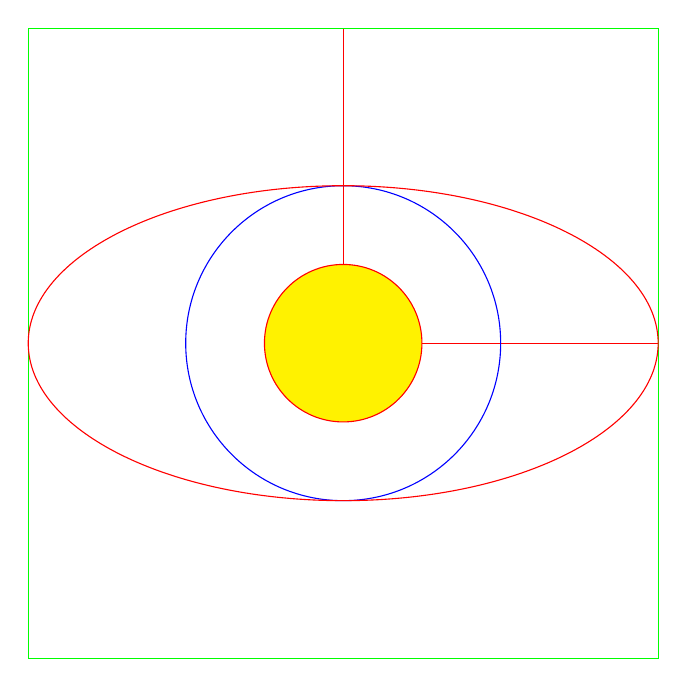
\begin{tikzpicture}
\draw[red] (0,0)--(4,0)--(4,4)--(0,4)--cycle;
\draw[blue] (0,0) circle [radius=2];
\draw[green] (-4,-4) rectangle (4,4);
\draw[red] (0,0) ellipse [x radius=4,y radius=2];
\filldraw[fill=yellow,draw=red] (0,0) circle [radius=1];
\end{tikzpicture}
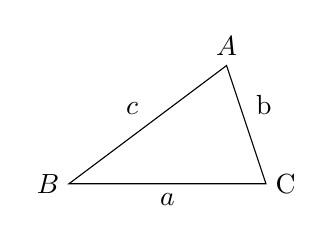
\begin{tikzpicture}
\draw (2,1.5) node[above] {$A$} -- node[above left] {$c$} (0,0) node[left]{$B$}--node[below]{$a$}(2.5,0)node[right]{C}--node[above right]{b} cycle;
\end{tikzpicture}\\
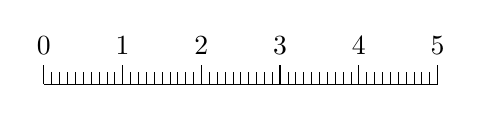
\begin{tikzpicture}
\draw (0,0)--(5,0);
\foreach \i in{0.1,0.2,...,5.0}{\draw[very thin](\i,0)--(\i,0.15);}
\foreach \I in{0,1,2,3,4,5}{\draw (\I,0)--(\I,0.25) node[above] {\I};}

\end{tikzpicture}\\
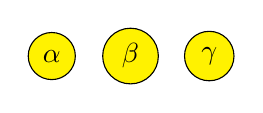
\begin{tikzpicture}
\foreach \n/\t in{0/\alpha,1/\beta,2/\gamma}{\node[circle,draw,fill=yellow] at (\n,0) {$\t$};}
\end{tikzpicture}
\end{document}
   